\section{Experimental protocols and full results}
\label{sec:evaluation-details}
This appendix records task construction, metrics and full results for the three evaluation questions. Appendix~\ref{sec:supporting-studies} collects the supporting ablations, maintenance studies and diagnostics.

\subsection{Transfer to an independently maintained retail environment}
We use Sierra's retail environment from $\tau$-bench~\cite{taubench} as an external source of independently authored test annotations, synthetic order records, and executable business tools. We deterministically select 15 different target orders from 12 annotated test tasks. We preserve the annotated item and refund parameters for returns and the annotated cancellation inputs where available. The adapter calls the unmodified order lookup, address update, return, and cancellation functions. It projects the replies to the agent's view and uses fixed requests and simulated confirmations.

We construct state pairs for testing the delivery boundary. The same request initially authorizes updating the alternate address on a pending order. In the changed variant the simulator marks it delivered at a preassigned model turn. Some requests allow an annotated return; others require a safe stop. A third family first commits the cancellation of a separate order before the target order changes. The external benchmark supplies the retail tools and task material. The address-update branch, state schedule, conditional authorizations, and privacy scorer are part of our adaptation.

We compare agent-directed reads under the original task-level authorization, a composable refreshed route table, and the versioned contract backend. All arms share the same Qwen4-Max endpoint, prompts, tools, authority, confirmation and recovery policy. Thirty derived tasks and three repetitions per arm give 270 runs. We assess raw field releases against the currently valid route and score success from the upstream tool's actual simulated state changes and expected safe stops. The bounded cohort tests transfer of the enforcement mechanism to another tool implementation.

\begin{table*}[t]
\centering
\small
\begin{tabular}{@{}lrrrrrr@{}}
\toprule
Read policy & Correct & Excess fields & Block recovery & Calls through outcome & Calls after closure & Approvals\\
\midrule
Agent-directed & 90/90 & 270 & -- & 825 & 0 & 105\\
Refreshed route table & 90/90 & 0 & 45/45 & 780 & 0 & 105\\
Versioned contracts & 90/90 & 0 & 45/45 & 780 & 1 & 105\\
\bottomrule
\end{tabular}
\caption{Retail transfer study. Correct outcomes include 15 expected safe stops per arm. Block recovery is conditional on a denied field read. All arms produce 90 normal final replies.}
\label{tab:external-retail}
\end{table*}

The delivery event falls between read preparation and attempt in all 45 state-change runs per arm. Agent-directed reads deliver six obsolete address fields per changed run. Its confirmation check then sees that the address update is unavailable, so the agent still recovers. Both guarded arms stop the field release one tool call earlier. Each reduces observed excess fields from 270 to zero and saves 45 calls through the business outcome. The two guards match on correctness, excess exposure, and business-stage tool calls. All three arms deliver the prescribed safe stop on all 15 such runs. The result extends the observed delivery-time effect to independently developed retail tools, under our controlled state schedule. It does not estimate a passive rate of state changes or imply a score on the original benchmark protocol.

\subsection{Gaia2 delivery-window protocol and results}
\label{sec:gaia-delivery-details}

We use three previously exercised public Adaptability tasks (0863, 0913 and 0924) and seeds 19, 113 and 421. We retain the original tasks, native tools and cancellation event, and use the upstream business scorer. The harness starts a common auxiliary catalog read after the first checkout while the original item is still eligible. It saves the exact identifier and the current version. After the first report, it waits up to 90 seconds for the native cancellation and attaches the pending result or denial to a tool reply. We count the pending reply when the model receives it. The agent issues all business calls, and the auxiliary read is excluded from native tool-call totals.

The timing comparison runs three arms (27 assignments). The agent-directed arm returns the pending result, and the preparation-time route table validates the read against the state at which the auxiliary read begins. The release-time contract compares the saved version with the version at delivery. Two assignments fail the upstream first-stage check before cancellation and remain in the all-assignment success denominator. Both Gaia2 comparisons use Qwen4-Max, with common prompts and budgets across arms within each comparison.

\begin{table*}[t]
\centering
\small
\begin{tabular}{@{}lrrrrr@{}}
\toprule
Read policy & All passed & Window reached & Stale replies & Matched passed & Matched post-switch calls\\
\midrule
Agent-directed & 8/9 & 8/9 & 8/8 & 7/7 & 52\\
Route table at preparation & 9/9 & 9/9 & 9/9 & 7/7 & 53\\
Contract at delivery & 8/9 & 8/9 & 0/8 & 7/7 & 55\\
\bottomrule
\end{tabular}
\caption{Gaia2 timing comparison. Stale-reply denominators are the runs that reached the delivery window. Among the seven matched triplets, stale replies number 7, 7 and 0. All eight denials in the contract arm are followed by task success.}
\label{tab:gaia-window-details}
\end{table*}

The strengthened-table comparison uses the same three tasks and seeds (18 assignments, 36 model responses allowed per run). Both arms keep their preparation check. The strengthened table also resolves the route from fresh state before delivery. Both arms use the same denial text. One table run fails to trigger cancellation, leaving eight matched pairs. The corresponding contract run reaches the window and blocks the reply before later reaching its response limit. The two matched contract failures occur on task 0913 at seeds 113 and 421. In the six pairs in which both arms pass, post-switch native calls total 43 for the table and 42 for the contract. Across all eight matched pairs, total model responses are 134 and 158, respectively, including responses before the switch.

\begin{table*}[t]
\centering
\small
\begin{tabular}{@{}lrrrrr@{}}
\toprule
Delivery check & All passed & Window reached & Stale replies & Matched passed & Matched post-switch calls\\
\midrule
Refreshed route table & 8/9 & 8/9 & 0/8 & 8/8 & 59\\
Contract & 6/9 & 9/9 & 0/9 & 6/8 & 58\\
\bottomrule
\end{tabular}
\caption{Gaia2 comparison with both checks at delivery. Paired columns condition on both runs reaching the delivery window. The all-assignment columns retain the run without a cancellation.}
\label{tab:gaia-refresh-details}
\end{table*}

\subsection{Refund grant dependencies and matched rerun}
\label{sec:refund-binding-details}

We hold the hosted Qwen4-Max model, tools, authorization, confirmations, feedback, and scoring fixed across the broad contract, narrow contract, and strengthened route table. Each arm runs the same five synthetic trajectories at three seeds (45 runs overall). The trajectories cover bank-to-wallet-to-bank with continuous bank authorization and unchanged bank fields, an unrelated note update, revocation followed by renewed authorization, a changed bank reference, and wallet remaining the preferred route. Every run reaches the pending-grant decision and a correct single refund.

Continuous authorization and unchanged input values make reuse valid in the first two trajectories. The other three must reject the old read. The narrow contract retains scope and single-use checks and binds continuity of the bank authorization and the versions of the exact requested fields. The strengthened table checks the same authorization generation and field versions at delivery. Table~\ref{tab:refund-binding-details} reports the matched decisions and calls.

\begin{table*}[t]
\centering
\small
\begin{tabular}{@{}lrrr@{}}
\toprule
Measure & Refreshed route table & Broad contract & Narrow contract\\
\midrule
Correct refunds & 15/15 & 15/15 & 15/15\\
False releases among obsolete reads & 0/9 & 0/9 & 0/9\\
Unnecessary denials among valid reads & 0/6 & 3/6 & 0/6\\
Valid grants reused & 6 & 3 & 6\\
Reads prepared again & 9 & 12 & 9\\
Tool calls after pending-read decision & 66 & 78 & 66\\
Total tool calls & 126 & 138 & 126\\
\bottomrule
\end{tabular}
\caption{Qwen4-Max refund rerun. All 15 task-seed matches reach the grant decision in every arm. The three denials unique to the broad contract occur when the wallet briefly becomes preferred and the bank route subsequently becomes eligible again.}
\label{tab:refund-binding-details}
\end{table*}


\subsection{Autonomous model experiment}
\label{sec:autonomous}
We compare three policies. \textsc{Upfront} returns all task-authorized candidate inputs in its first state inspection. \textsc{Agent only} lets the model request inputs as needed while preserving task-level authorization and common plan and execution checks. A shadow check records when a request would violate step-level necessity. \textsc{State guard} enforces necessity at delivery. The upfront arm isolates an eager-release policy and should be interpreted separately from the dedicated AirGap-style adaptation.

The main experiment consists of 120 parameterized synthetic tasks across refund and logistics, grouped into 60 pairs. Paired members share the user request, profile and rules, with different business state. The suite balances single-route, route-switch and multiple-stage workflows, 40 of each. We run all three policies with each of two hosted model aliases (\texttt{qwen3.8-flash} and \texttt{qwen4-max}), native tool calls and shared task authorization, approval and recovery rules. Each task runs with three seeds, yielding 360 attempts per policy. The archived protocol fixes temperature 0.3, a budget of 40 model responses, a 512-token output cap per response, and two recoveries. We retain incomplete attempts and distinguish HTTP retries from returned model calls.

In route-switch tasks, the simulated condition can change after the first read justification and before field delivery. The event occurred in all 120 attempts in each on-demand arm for both models. In the upfront arm it occurred in 108 of 120 Qwen3.8-Flash attempts and all 120 Qwen4-Max attempts. Some Qwen3.8-Flash workflows used already supplied values and skipped the triggering action. Event exposure in the upfront comparison therefore varies by model. The primary comparison uses the two on-demand arms.

\paragraph{Metrics and uncertainty.}
An independent task ledger determines successful business effects and applicable confirmations. We separately count unique raw field instances (deduplicated within an attempt), fields unused by the resulting valid execution, and fields released despite a stale evidence check. These counts may overlap. We count successful business effects even when the expected final answer fails to arrive, and report final-answer completion separately. We check visible model prose and simulated external text for exact synthetic value matches. The protocol does not observe paraphrases, partial disclosures, or hidden reasoning. Intervals use 5,000 paired cluster bootstrap draws over the 60 state pairs, with both members and all repeats kept together. They describe uncertainty for this constructed suite, rather than a production workload.

\begin{table*}[t]
\centering
\small
\begin{tabular}{@{}lrrrrrrrr@{}}
\toprule
Policy & Business success & Raw fields & Unused & Stale & Tool calls & Model calls & Approvals & Leaks \\
\midrule
Upfront & 359/360 & 1752 & 1049 & 1 & 2775 & 3134 & 139 & 1 \\
Agent only & 359/360 & 850 & 144 & 144 & 3487 & 3840 & 141 & 0 \\
State guard & 359/360 & 707 & 0 & 0 & 3446 & 3806 & 141 & 1 \\
\bottomrule

\end{tabular}
\caption{Autonomous comparison across 360 attempts per policy and model (2,160 total). Field instances are deduplicated within attempts and summed. Leaks counts trajectories with a visible exact-value disclosure. Approvals are simulated. Repeated HTTP transport attempts are excluded from the model calls column.}
\label{tab:autonomous}
\end{table*}

\begin{figure*}[t]
\centering
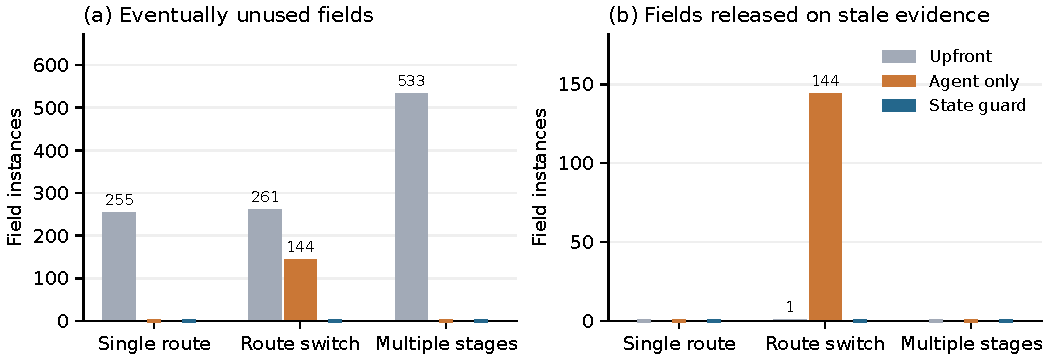
\includegraphics[width=.92\textwidth]{figures/exposure.pdf}
\caption{Qwen3.8-Flash field exposure by workflow family (120 attempts per policy per family). Zero counts appear as short marks on the baseline. Panels use distinct vertical scales. The state event triggered in all on-demand route-switch attempts and in 108 of 120 upfront attempts.}
\label{fig:exposure}
\end{figure*}

\subsection{Autonomous results}
For Qwen3.8-Flash, Table~\ref{tab:autonomous} shows that state enforcement reduced the raw fields delivered to the model from 850 to 707 relative to agent-only reads (16.8\%). It eliminated the 144 observed stale-field instances and the 144 eventually unused field instances of that comparator. Figure~\ref{fig:exposure} localizes the stale-field difference to route-switch cases. In the static and multiple-stage cases, agent-only already achieved zero eventually unused field instances.

The guard blocked 120 read attempts, and 119 of the corresponding trajectories completed the business task. Aggregate completion was 359/360 for each policy. Within route switches, agent-only completed 120/120 and the guard completed 119/120. The failures differed across policies, so similar aggregate success does not imply identical trajectories. Normal final responses accompanied 354, 352 and 355 attempts in upfront, agent-only and guard respectively.

The guard-minus-agent-only difference in stale field instances was $-0.400$ per attempt (95\% interval $[-0.550,-0.258]$). The business success difference was 0 percentage points (interval $[-0.83,0.83]$ points). Tool and model calls fell by 41 and 34 in total. The tool difference interval was $[-0.617,0.372]$ calls per attempt and the model difference interval was $[-0.583,0.386]$. These intervals leave the direction of the cost difference unresolved. Approval counts were equal in the two on-demand arms.

One upfront and one guard attempt exposed a value in final prose. In the guard attempt, the value had been legitimately obtained for the workflow. There were no exact matches in the simulated external delivery logs. This distinction illustrates why preventing unnecessary reads and controlling what an agent repeats require separate evaluation.

\paragraph{Replication with Qwen4-Max.}
The state guard again reduces stale field instances from 144 to zero relative to agent-directed reads, and all three arms complete 360/360 workflows. All 120 blocked-read runs recover. The guard uses five additional tools (3,051 versus 3,046), a paired difference of 0.014 per run with a 95\% interval of $[-0.008,0.042]$. We observe no exact-value disclosure in visible text or simulated egress in any arm. The upfront arm releases 1,044 fields unused by the eventual valid execution.

\section{Supporting ablations, maintenance and diagnostics}
\label{sec:supporting-studies}
\subsection{Scripted comparison with refreshed route tables}
\label{sec:scripted}
We compare the two stronger backends using scripted decisions to isolate middleware behavior. The backends share authorization, confirmation, recovery and verification-reuse rules. Scenario definitions specify expected committed goals, fields and steps. Unsafe continuations, duplicate effects, and unexpected data delivery can thus be checked directly against the scenario. These studies run no model inference.

\begin{table}[t]
\centering
\small
\setlength{\tabcolsep}{2.2pt}
\begin{tabular}{@{}lrrrr@{}}
\toprule
Study & Done & Fields & Denials & Approvals \\
\midrule
Refund cases & 3/3 & 6 & 2 & 3 \\
Independent goals & 3/4 & 12 & 3 & 7 \\
Dependent goals & 5/6 & 17 & 1 & 9 \\
Signature rule (new) & 4/6 & 19 & 1 & 9 \\
Signature rule (regression) & 12/15 & 39 & 2 & 20 \\
\bottomrule

\end{tabular}
\caption{Scripted comparisons. Each row reports the identical counts observed for each backend separately. \emph{Done} counts fully completed workflows. The regression row includes previously expected safe stops.}
\label{tab:scripted}
\end{table}

\paragraph{Refund cases.}
We test restoration of the preferred refund route, reuse of identity verification across a plan change, and authorized access to exact quotes. Both backends handle all three cases. For one composition of refund and quote goals, the enumerated table requires three additional logical entries while the contract-based backend composes the existing contracts. This difference depends on the table representation.

\paragraph{Logistics composition and dependency.}
When the table can compose single-goal recipes, both backends execute new combinations of a pickup-site change and a time change with no configuration additions after freezing. We then let a pickup-site change invalidate a previous booking and require a different verification at the new site. An initial development trace revealed redundant site verification on replan. We give both backends a versioned reuse rule and freeze again. On six new composed cases, both complete five workflows and deliberately stop the unauthorized remaining appointment in the other. Each delivers 17 necessary field instances. A read of an obsolete time slot is denied by both. Table~\ref{tab:scripted} reports the matched counts.

\paragraph{A new business rule.}
We add a signature-authorization check for high-value rebooking. A valid existing slot can be retained without the check. The rule needs one manually written applicability declaration per backend after building migration adapters. In the contract system the declaration targets the two rebooking tools. In the table it targets a reusable rebooking fragment. Both expand it across four existing route variants and generate four variants requiring the check. This measures authored records for this design. Adapter development and maintenance time remain unmeasured.

Across 30 prior regression runs (15 per backend), seven recorded metrics agree with the corresponding prior runs, and no signature input is delivered. On six new cases per backend, each completes four workflows. In the others, a needed field is unauthorized or no alternate slot is available. Both preserve the completed pickup-site change. They deliver 19 field instances each, all within the case-defined required set. When a preferred slot returns after signature verification, both reject the old slot read and reuse the valid verification. Focused checks show that missing or stale signature authorization blocks delivery of reservation inputs.

\subsection{Autonomous comparison with a refreshed route table}
\label{sec:strong-autonomous}
We compare the composable route table and the contract verifier on 60 new state pairs (120 synthetic tasks). Three repetitions per backend give 720 runs with the same hosted Qwen3.8-Flash alias. The design matches tools, authorization, confirmation and recovery across backends. A business checkpoint schedules changes independently of raw read requests. It includes return of a preferred route, a change after a committed effect, and loss of all authorized continuations. A separate condition updates the evidence version while keeping the same route admissible. Appendix~\ref{sec:autonomous-protocol} describes the protocol.

\begin{table*}[t]
\centering
\small
\begin{tabular}{@{}lrrrrrrr@{}}
\toprule
Backend & Correct & Excess & Recoveries & Raw fields & Tool calls & Model calls & Approvals\\
\midrule
Refreshed route table & 360/360 & 0 & 177/177 & 630 & 5,000 & 5,356 & 420\\
Versioned contracts & 359/360 & 0 & 265/265 & 629 & 5,125 & 5,490 & 419\\
\bottomrule
\end{tabular}
\caption{Autonomous comparison on Qwen3.8-Flash. Correct outcomes include 60 expected safe stops per arm. Recovery is conditional on a blocked read. All 177 matched runs blocked by both backends achieved the correct outcome in both arms.}
\label{tab:strong-autonomous}
\end{table*}

Both backends recorded zero excess field releases and zero exact-value disclosure in visible model text. The one incorrect outcome was a contract-arm run that changed the pickup point then received an HTTP 400 before booking. In 90 matched runs with unchanged route eligibility and an updated evidence version, the contract arm recorded 85 evidence-expiration denials. The two arms used 1,219 and 1,423 tools respectively. Over all tasks the contract-minus-table paired mean difference is 0.347 tool calls, with a 95\% task-pair bootstrap interval of $[-0.308,0.961]$. These observations identify a recovery cost when version binding is stricter than current eligibility. They show no incremental reduction in excess releases on this suite.

\paragraph{Replication with Qwen4-Max.}
We repeat all 720 assignments with the same tools, task pairs, seeds and budgets. Both arms produce 360/360 correct outcomes, zero excess field releases and zero visible exact-value disclosures. The table recovers after all 180 read blocks. The contract arm recovers after all 270, including 90 denials where evidence versions changed and the route remained eligible. Total tool calls are 10,867 and 10,885 respectively. Through the terminal business outcome, the counts are 3,810 and 4,170. All 360 additional pre-closure calls occur in the 90 version-only runs. Another 7,057 and 6,715 calls occur after workflow closure (Figure~\ref{fig:strong-stage-cost}). Normal final replies occur in 121 and 122 runs; all 45 gateway interruptions follow a correct business outcome. The execution ledger and the dialogue endpoint measure distinct aspects of agent performance.

\begin{figure*}[t]
\centering
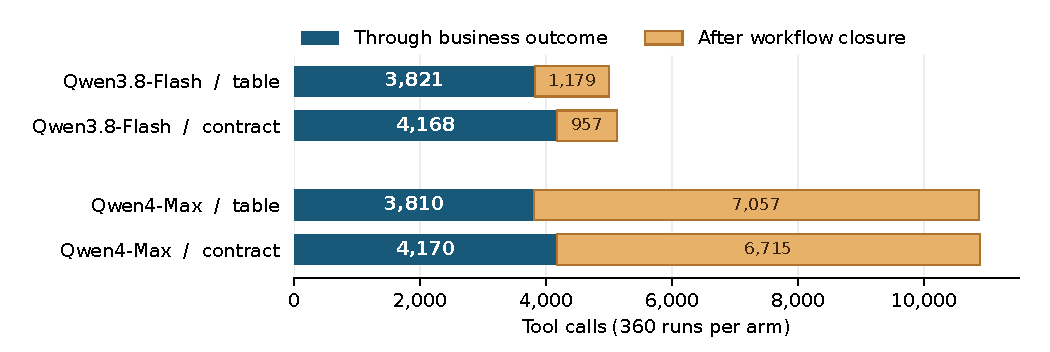
\includegraphics[width=\textwidth]{figures/strong-call-stages.pdf}
\caption{Tool calls through the business outcome and after workflow closure for the strong-baseline comparison. The shared original tool protocol remains in force for both models. The after-closure segment accounts for most of the Qwen4-Max aggregate cost.}
\label{fig:strong-stage-cost}
\end{figure*}

\subsection{Rule maintenance and audit}
We add three business rules covering changed bank details, cross-region pickup moves and restricted-site bookings. Both backends use three authored rule declarations. The table names three reusable recipe fragments. The contract configuration names four tools. The table additionally regenerates four existing and four new recipe entries. Both share the same generated business operation catalog. Both pass 36 policy fixtures, retain behavior on 12 old paths per backend, and detect all 15 injected faults per backend. Faults cover missing rules, selector changes, condition reversal, wrong field binding and missing prerequisites. The results measure configuration artifacts and regression coverage. Human authoring time and natural misconfiguration rates remain open.

Each backend emits enough information to reconstruct eight curated decisions after we add a shared structured log. It records rule identifiers, requested fields, prerequisites, and current and prepared evidence versions. Native contract logs include successful reads, while neither native interface carries the rule identifier in these cases. A separate reconciliation of approved rules and deployed configuration pinpoints all 15 faults per backend. The audit result therefore supports explicit instrumentation and configuration reconciliation for either implementation.

\subsection{Exploratory second-model compatibility}
A matched pilot runs six strong-baseline tasks with both backends using Qwen4-Max and compares the corresponding Qwen3.8-Flash records under the same tool protocol and budgets. Each model achieves 12/12 correct business outcomes and zero excess field releases. Qwen4-Max produces a normal final reply in 5/12 runs, compared with 12/12 for Qwen3.8-Flash. Tool calls rise from 158 to 340, with after-completion calls rising from 22 to 204. In this pilot the extra calls arise after the business outcome is settled. The strong-backend replication is reported in Section~\ref{sec:strong-autonomous}. Sections~\ref{sec:airgap-adaptation} and~\ref{sec:factorial} report the remaining replications. Token limits and finishing behavior are tracked separately from business completion.

In a separate matched diagnostic on six other tasks, we change only the response to a tool call after the workflow is closed. Both feedback formats achieve 12/12 correct business outcomes and zero excess releases. Explicit closure feedback increases normal final replies from 4/12 to 12/12 and cuts after-closure calls from 225 to 8. Calls before closure total 136 in each condition. This diagnostic isolates a tool-protocol effect on observed cost and is recorded separately from the full replication.

\subsection{Upfront minimization with escalation}
\label{sec:airgap-adaptation}
We evaluate a study-specific AirGapAgent-style adaptation with base-context minimization, a restricted conversational view and user escalation when additional fields are needed. The two on-demand arms begin with no private field values. The protocol uses 72 variants comprising 18 business-state pairs with both clean and externally injected tool text, two models, three arms and three repetitions (1,296 runs). This tests the adaptation on our workflows. The original AirGapAgent benchmarks and reported scores use different tasks and metrics.

\begin{table*}[t]
\centering
\small
\begin{tabular}{@{}llrrrrrr@{}}
\toprule
Model & Method & Correct & Unused & Data escalations & Action approvals & Tool calls & Model calls\\
\midrule
Qwen3.8-Flash & AirGap-style & 216/216 & 576 & 112 & 222 & 1927 & 2580\\
              & Agent only   & 216/216 & 0   & 0   & 222 & 1793 & 2011\\
              & State guard  & 216/216 & 0   & 0   & 222 & 1792 & 2012\\
Qwen4-Max     & AirGap-style & 216/216 & 366 & 182 & 222 & 2249 & 2896\\
              & Agent only   & 216/216 & 0   & 0   & 222 & 1900 & 2116\\
              & State guard  & 216/216 & 0   & 0   & 222 & 1963 & 2176\\
\bottomrule
\end{tabular}
\caption{AirGap-style adaptation and two on-demand controls. Unused fields are raw fields observed by the conversational agent that are outside the gold route field set. Data escalations ask for an additional field. Action approvals confirm the business operation.}
\label{tab:airgap-adaptation}
\end{table*}

Both on-demand arms eliminate observed unused fields in this study. The adaptation releases 576 and 366 unused field instances per model. With Qwen4-Max, the guard reduces tool calls by 286 and data escalations by 182 relative to the adaptation. All arms complete 216/216 tasks and preserve equal action approval counts. The exact-value checker finds no observed leakage and no unauthorized values delivered to the conversational agent. This comparison shows the effect of postponing disclosure under these policies. The separate stale-read settings in Sections~\ref{sec:autonomous} and~\ref{sec:strong-autonomous} test the need and cost of runtime enforcement.

\subsection{Query-order and enforcement ablation}
\label{sec:factorial}
A $2\times2$ study separates fixed versus planned predicate-query advice from advisory versus enforced reads. The contract and trusted predicates are shared. Each model uses three repetitions on 12 tasks per arm. We reproduce both archived versions of this study, one with native tool calls and one with JSON tool calls in model text, for 576 runs across models and interfaces. Table~\ref{tab:factorial} shows the Qwen4-Max replication.

\begin{table*}[t]
\centering
\small
\begin{tabular}{@{}lllrrrr@{}}
\toprule
Interface & Query advice & Read check & Correct & Stale fields & Predicate queries & Tool calls\\
\midrule
Native & Fixed   & Advisory & 36/36 & 12 & 12 & 292\\
       & Fixed   & Enforced & 36/36 & 0  & 12 & 294\\
       & Planned & Advisory & 36/36 & 12 & 9  & 288\\
       & Planned & Enforced & 36/36 & 0  & 9  & 291\\
Text   & Fixed   & Advisory & 36/36 & 12 & 12 & 344\\
       & Fixed   & Enforced & 36/36 & 0  & 12 & 348\\
       & Planned & Advisory & 36/36 & 12 & 9  & 345\\
       & Planned & Enforced & 36/36 & 0  & 10 & 340\\
\bottomrule
\end{tabular}
\caption{Qwen4-Max query-order and enforcement ablation. Stale fields are values delivered after the evidence supporting the read changed. Advice concerns the order of obtaining trusted predicates.}
\label{tab:factorial}
\end{table*}

Both models reproduce the twelve-to-zero stale-field contrast at each advice setting and in each interface. Qwen4-Max reaches 36/36 in every arm. With Qwen3.8-Flash, the same native arms achieve 36/36 and the archived text arms range from 33/36 to 34/36. Planned advice saves two to three predicate queries in the Qwen4-Max arms relative to fixed advice. Deployment conclusions about query cost remain bounded by the small predicate suite and its configured priors. The read check supplies the observed privacy effect in this ablation.

\subsection{Delivery-window and refund-rule maintenance studies}
\label{sec:refund-maintenance}
\paragraph{Is a decision at read preparation sufficient?}
We use three public Gaia2 Adaptability tasks~\cite{gaia2data} with upstream cancellation events and business scoring. After an initially valid catalog read starts, the experiment holds its reply until the original order cancellation. Qwen4-Max chooses all business actions. In seven same-task, same-seed triplets that reached the delivery window, agent-directed reads and a table refreshed at read preparation each delivered seven stale catalog replies. A contract checked at delivery returned zero stale replies and all three policies completed seven tasks. This is a controlled exposure opportunity on previously used public tasks. The outcome concerns the pending reply, including possible repeated delivery of an already observed identifier.

In a second run, the table also rechecked at delivery. Neither implementation delivered stale replies in the eight pairs that reached the window. The table completed eight and the contract six. Both generated the same value-free denial, and the two matched contract failures exhausted the response budget before the final user report. The paired post-switch tool totals were 59 and 58. These comparisons locate the benefit at the delivery boundary and leave production frequency unmeasured.

\paragraph{Which evidence should invalidate a pending read?}
We run Qwen4-Max on five synthetic refund trajectories with three seeds and three backends. A temporary wallet-priority change that returns to bank leaves bank authorization and the requested field versions intact. Binding all plan-support versions rejects three still-valid reads in this case. The narrower grant binds the bank authorization generation and the requested field versions, with current-route checking at delivery. It rejects all nine obsolete reads, reuses all six valid reads, and removes twelve downstream tool calls. The strengthened table, which also checks authorization generation and field versions, matches the narrow contract on all 15 pairs. All arms complete 15/15 refunds.

\begin{table}[t]
\centering
\small
\begin{tabular}{@{}lrr@{}}
\toprule
Metric & Table & Contract \\
\midrule
Workflow checks passed & 256/256 & 256/256 \\
Excess release cases & 0 & 0 \\
New authored declarations & 3 & 3 \\
Generated route recipes & 12 & 0 \\
Unchanged legacy checks & 32/32 & 32/32 \\
Structured decisions explained & 7/7 & 7/7 \\
Injected faults localized & 3/3 & 3/3 \\
\bottomrule
\end{tabular}
\caption{Refund rule changes under shared compilation and audit logging. Correct workflow checks include expected safe stops.}
\label{tab:refund-rule-maintenance}
\end{table}

\paragraph{What changes when business rules compose?}
We add three conditional checks to both the narrow contract and a composable table. Enhanced verification can serve both refund routes. A changed beneficiary adds a bank-only check. A large refund requires enhanced verification and review, and review waits for the beneficiary check when applicable. We freeze a factorial suite of four route states, eight trigger combinations, and eight field-authorization sets. A separate scripted ledger scores committed route, ordered prerequisites, released fields and approval. Table~\ref{tab:refund-rule-maintenance} summarizes the comparison. Both backends pass all 256 cases, committing 88 refunds and stopping safely in 168. The observed fields remain within the approved requirements in every case.

Both implementations use three authored overlay declarations with five route references and three dependency references. The shared compiler generates 31 action entries per backend from two original entries. It also materializes 12 table recipes from two original recipes, while the contract execution uses its action registry. The original authored entries remain intact. Bank-only, wallet-only and wallet-preferred flows require regression under the new rules. We also retain the no-route stop as a common check. With the new conditions disabled, all 32 legacy cases per arm preserve their prior outcomes and fields.

With a shared structured log, both implementations reconstruct all seven curated decisions, including valid composition, route change, authorization revocation, changed field version, an out-of-scope request, and a missing prerequisite. None of the five denied reads in either arm releases a raw value. Comparing approved declarations with deployed configuration locates each of three symmetric injected faults, and the corresponding regression supplies a counterexample. This study measures authored declarations, emitted artifacts and scripted diagnostic coverage. The shared compiler and log schema are setup costs, and developer time and naturally occurring mistakes remain open.

